\documentclass[a4paper,landscape,10pt]{cheatsheet}

\usepackage[spanish]{babel}
\usepackage[utf8]{inputenc}
\usepackage{physics}
\usepackage{amsmath}
\usepackage{bookmark}
\usepackage{amsfonts}
\usepackage{amssymb}
\usepackage{mathtools}
\usepackage{graphicx}
\usepackage{float}
\usepackage[rightcaption]{sidecap}

%addtolength{\oddsidemargin}{.875in} addtolength{\evensidemargin}{.875in} addtolength{\textwidth}{1.75in}
%addtolength{\topmargin}{.875in} \addtolength{\textheight}{1.75in}

\title{Physical biology}
\author{David Caro}
\date{08-01-2024}

\pdfinfo{%
  /Title    (Physical biology)
  /Author   (David Caro)
  /Creator  (David Caro)
  /Producer (David Caro)
  /Subject  (Physics)
  /Keywords ()
}

\begin{document}
\maketitle

%%%%%%%%%%%%%%%%%%%%%%%%%%%%%%%%%%%%%%%%%%%%%%%%%%%%%%%%%%%%%%%%%%%%%%%%%
\section{1.1 Life}
Common description uses 5 characteristics:
\begin{itemize}
  \item made of cells
  \item they replicate
  \item they evolve
  \item store information (genes)
  \item use energy
\end{itemize}

\hfill\\
\section{1.2 Cellular theory}
\begin{itemize}
  \item 1665 Hook -> first microscope -> \textbf{dead cells}\\
  \item 1660-1680 Van Leeuwenhoek -> more potent microscopes -> \textbf{live cells and microorganisms}\\
  \item 1831 Brown -> \textbf{defines the nucleus}\\
  \item 1838 Schleiden (for plants), 1839 Schwann (for animals) and 1857 Virchow define the cellular theory:
        \begin{itemize}
          \item The cell is the unit of structure for life
          \item Cells retain a dual existence as individuals and building blocks
          \item (Virchow 1857) All cells come from other cells
        \end{itemize}
\end{itemize}

\hfill\\
\section{1.3 Theory of evolution}
Darwin and Wallace create the theory of evolution, two main principles:
\begin{itemize}
  \item All species are related by common ancestors.
  \item Characteristics of species change from generation to generation.
\end{itemize}
The key insight was their description of the process that pushes for that change: \textbf{natural selection}.\\
This means that you can draw a \textbf{tree of life} from the common ancestor to the current extant species.

\hfill\\
\section{1.4 Chromosomic theory of inheritance and central dogma}
Chromosomes are made of a single DNA molecule, and some of it's segments that codify the products in the cell are called
genes.\\
The central dogma of microbiology states that the flow of information is unidirectional:
\begin{itemize}
  \item DNA
  \item -transcription-> mRNA
  \item -traduction-> protein
  \item -> specific trait
\end{itemize}

\hfill\\
\section{1.5 Taxonomy}
Naming organisms, started by Carl Linnaeus, binomial system, ex:\\
\begin{center}
  <gender> <species>: quercus robur (oak)
\end{center}
Added a hierarchy of taxonomical groups:\\
\begin{center}
  species < gender < family < order < class < phylum < kingdom
\end{center}
Can be drawn for all species in a phylogenetic tree, where the closest the branch, the more closely related the
species.\\
Recent genetic studies have shown that this is obsolete, and currently life is classified in three domains:
\begin{itemize}
  \item Bacteria
  \item Archaea
  \item Eukarya (cells with well defined nucleus, plants, fungi, animals, ...)
\end{itemize}

\section{2.0 Biomolecules}
There's organic and inorganic molecules that are part of a living being, we will focus on the organic ones:

\hfill\\
\section*{2.1 Proteins}
Polymers of aminoacids joined by peptide bonds, structure of an aminoacid:
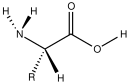
\includegraphics{images/amino_acid_structure}\\
{\footnotesize by Smokefoot - Own work, Public Domain, https://commons.wikimedia.org/w/index.php?curid=106539890}\\
Note the amino group $NH_2$, the carboxyl acid group $COOH$, and the lateral chain with the root $R$, characteristic of
every aminoacid.\\
They are joined by condensation, when the $COOH$ group creates a peptidic bind with the $NH2$ of the next.

\hfill\\
\section*{2.2 Protein structure}
There's 4 structure levels:
\begin{itemize}
  \item Primary: peptidic bonds between single aminoacids in the protein
  \item Secondary: hydrogen bonds between the $O$ of a $COOH$ group in one aminoacid and the $NH_2$ of another, can
        create two different shapes:
        \begin{itemize}
          \item $\alpha$-helix - $R$ groups facing outwards
          \item $\beta$-sheet
        \end{itemize}
        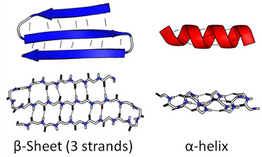
\includegraphics[width=0.2\textwidth]{images/secondary_protein_structure.png}
  \item Tertiary: \textbf{when $R$ groups are involved}, there's many kind of folds, but only a few bonds that can
        happen:
        \begin{itemize}
          \item \textbf{Hydrogen bonds} between $COOH$ carbonyl group and the lateral chain
          \item \textbf{Hydrogen bonds} between two lateral chains or $R$ groups
          \item \textbf{Covalent bonds}, commonly di-sulfur bridge between cysteine $R$ groups
          \item \textbf{Ionic bonds} between $R$ groups
          \item \textbf{Hydrophobe interactions and van der Waals forces}, when in water, the hydrophile lateral chains
                push the hydrophobe $R$ groups together, and then van der Waal forces keep them stable
        \end{itemize}
  \item Quaternary: Combination of polypeptide, bound by similar bonds than the tertiary structures.
\end{itemize}
Folding is often facilitated by a specific type of proteins called \textbf{chaperones}. These molecules are generated in
big quantities when there's a high rise in temperature. They attach themselves to the hydrophobe sections of unfolded
proteins to prevent other molecules from attaching and allow the protein to re-fold itself before any unfolded
aggregates get created.


\hfill\\
\section*{2.3 Protein function}
The functionality of a protein is strongly related to it's folding, two proteins with the same aminoacid sequence cat
behave really differently, for example prions are proteins that when folded in a specific way, become infectious.\\
When a protein loses it's folding it's said it gets \textbf{denaturated}, this can happen for many reasons (heat, pH,
...).\\
They are the more versatile of the molecule groups, having many functions:\
\begin{itemize}
  \item \textbf{Catalytic/enzymes}: they speed up many chemical reactions.
  \item \textbf{Defensive}: Antibodies and other proteins attack and destroy viruses and bacteria
  \item \textbf{Movement}: Motor protein and contractile proteins move substances within the cell, the cells themselves
        and the whole body (muscles).
  \item \textbf{Signaling}: They are involved in the transport and reception of signals, sometimes bound to the cell
        membrane to interact with neighboring cells.
  \item \textbf{Structural}: collagen of the skin and tendons, membrane proteins.
  \item \textbf{Transport}: They allow that some molecules enter and leave the cell, or transport them throughout the
        body (hemoglobin).
\end{itemize}

\hfill\\
\section*{2.4 Nucleic acids}
Formed by \textbf{nucleotides}: a pentose sugar (ribose with $OH$ on 2'/deoxyribose with $H$ on 2'), a nitrogenous base
(bound to the carbon 1'), and a phosphate (bound to the carbon 5').\\
Note that \textbf{nucleoside} is just the pentose sugar and the base.\\
Bases can be one of:
\begin{itemize}
  \item Cytosine - Pyrimidine
  \item Uracil (RNA)/Thymine (DNA) - Pyrimidine
  \item Guanine - Purine
  \item Adenine - Purine
\end{itemize}
The nucleotides are bound with phosphodiester bonds (covalent bonds) on 5' and 3', and form a directed chain, always
written from the nucleotid with the phosphate (5') free, to the one with the $OH$ (3') free.\\
That is also the direction they are synthesized.\\

They form two main structures:
\begin{itemize}
  \item \textbf{RNA}:
        \begin{itemize}
          \item Sugar: ribose
          \item Bases: A-U, G-C
          \item Structure: simple strand
          \item Function: transport, structural, etc.
        \end{itemize}
  \item \textbf{DNA}:
        \begin{itemize}
          \item Sugar: deoxyribose
          \item Bases: A-T, G-C
          \item Structure: double helix strand bound by hydrogen bonds of the bases
          \item Function: carries the genetic information
        \end{itemize}
\end{itemize}

In order to polymerize the nucleotides, the potential energy of the nucleotides is increased by adding phosphates,
creating triphosphate nucleosides or \textbf{activated nucleotides}, then when they get polymerized they need water and
generate inorganic pyrophosphate. Ex. ATP (adenine + 2 phosphates -> adenosin triphosphate) \\

\hfil\\
\section*{2.5 DNA structure}
The \textbf{primary structure} of the nucleic acids is just the sequence of basis it's made of.\\
\hfill\\
The \textbf{secondary structure} is built by hydrogen bonds between the $R$ groups, and for DNA is an
\textbf{antiprallel double helix}, where the bases are matched only between complementary purines and pyrimidines (G-C
has 3 hydrogen bonds, A-T has two hydrogen bonds).\\
The helix (2 nm wide) does a turn (3.4 nm) every 10 base pairs (0.34 nm), where the two strands phase is not symmetric,
creating one small and one big gap between them.\\
\hfill\\
The \textbf{tertiary structure} DNA is usually packed with proteins, in eucaryotes these are histones, the bundle is
called \textbf{chromatin}, and it comes in two flavors, a more packed one that is not ready for transcription
\textbf{heterochromatin} and a lightly packed one ready for transcription, \textbf{euchromatin}.\\

\hfil\\
\section*{2.6 RNA structure}
The \textbf{primary structure}: same as DNA, it's the sequence of basis.\\
\hfill\\
The \textbf{secondary structure}: the most common is the stem loops (horquilla), where a single strand bends over itself
to create a loop and a double helix section with itself.\\
\hfill\\
The \textbf{tertiary structure}: secondary structures fold to generate a great variety of forms for RNA.\\

\hfil\\
\section*{2.7 RNA types}
There's three main types of RNA:\\
\begin{itemize}
  \item \textbf{mRNA (messenger RNA)}:
        \begin{itemize}
          \item Transports information from the nucleus to the cytoplasm
          \item Gets translated in the ribosomes to generate proteins
          \item Single strand
        \end{itemize}TOTAL   26 TiB   21 TiB   21 TiB  1.4 GiB   67 GiB  5.2 TiB  79.97
        15:43:15 TOTAL   26 TiB   21 TiB   21 TiB  1.4 GiB   67 GiB  5.3 T

  \item \textbf{rRNA (ribosomal RNA)}:
        \begin{itemize}
          \item It's a structural part of the ribosomes
          \item There's several types that form the small and big subunits of the ribosome along with proteins
          \item Single strand with secondary structure
        \end{itemize}

  \item \textbf{tRNA (transfer RNA)}:
        \begin{itemize}
          \item Transports aminoacids to the ribosome
          \item Simple strand with clover-like secondary structure
        \end{itemize}
\end{itemize}


\hfil\\
\section*{2.8 Carbohydrates}
Made out of \textbf{monosaccharides}, they are composed by carbon, hydrogen and oxygen and are mainly used either as
energy storage, or as structural molecules.\\
They have one carbonyl group ($C=O$), several hydroxyl ($-OH$) and a variable number of carbon-hydrogen bonds ($C-H$).\\
\begin{itemize}
  \item \textbf{monosaccharides}: simplest of sugars, made of a single strand of carbons, with a carbonyl group and one
        or more hydroxyl (ex. glucose, fructose, galactose).
  \item \textbf{disaccharides}: formed by two monosaccharides when the hydroxyl groups bond (by condensation) to form
        \textbf{O-glycosidic bonds} (ex. 2 x glucose -> maltose + $H2O$, glucose + galactose -> lactose + $H2O$)
  \item \textbf{oligosaccharides and polysaccharides}: for groups of 2-10 monosaccharides bonded by glycosidic bonds, we
        call them oligosaccharides, and when they have more monosaccharides, we call them polysaccharides. (ex. starch,
        cellulose, chitin, glycogen).
\end{itemize}

\hfill\\
\section*{2.9 Carbohydrates: polysaccharides}
They have mainly two functions, \textbf{structural} and \textbf{energy reserve}. They also have a role in cell
identification (ex. sperm attaching to the ovule). The main polysaccharides of life are:
\begin{itemize}
  \item \textbf{Starch}
        \begin{itemize}
          \item reserve molecule used by plants
          \item amylose and amylopectin (both made of $\alpha$-glucose)
          \item amylose has a lineal helix structure
          \item amylopectin has a ramified helix structure
        \end{itemize}
  \item \textbf{Glycogen}
        \begin{itemize}
          \item reserve molecule used by animals, fungi and some bacteria
          \item made of $\alpha$-glucose, very similar to amylopectin but it's even more ramified
        \end{itemize}
  \item \textbf{Cellulose}
        \begin{itemize}
          \item Structural support for plants and many algae
          \item parallel chains of $\beta$-glucose joined with hydrogen bonds
        \end{itemize}
  \item \textbf{Chitin}
        \begin{itemize}
          \item Structural support for insects and fungi
          \item parallel chains of NAG (N-acetylglucosamine) joined with alternating hydrogen bonds
        \end{itemize}
  \item \textbf{Peptidoglycan}
        \begin{itemize}
          \item Structural for bacteria
          \item parallel chains joined with peptide bonds (using a chain of 4 aminoacids from NAM)
          \item alternating NAG and NAM, N-acetylmuramaic acid, like NAG but with 4 aminoacids on C-3
        \end{itemize}
\end{itemize}


\hfill\\
\section*{2.10 Lipids}
Main characteristics (classified by their physical attributes, not chemical structure like polysaccharides):
\begin{itemize}
  \item Insoluble in water
  \item Soluble in organic solutions (ethanol, chloroform, ether, ...)
  \item Three main elements, \textbf{carbon, hydrogen and oxigen}, smaller amount of others \textbf{nitrogen,
          phosphorous, sulfur}.
  \item can be found bonding to other molecules with \textbf{covalent bonds (glucolipids)} or \textbf{non-covalent (lipoproteins)}.
\end{itemize}

Common ones (among others):
\begin{itemize}
  \item Phospholipids
  \item Triglycerides
  \item Steroids
\end{itemize}

\section*{2.11 Steroids}
Composed of 4 fused rings (steroid rings) and an isoprene. \\
Amphiphile  molecules.\\
Main functions:
\begin{itemize}
  \item Signaling - hormones (ex. testosterone)
  \item Structural - changing membrane fluidity (ex. cholesterol)
\end{itemize}

\section*{2.11 Triglycerides}
Composed of a glycerol molecule with 3 fatty acids attached with ester bonds (if 2 fatty acids -> diglyceride, if 1 monoglyceride)\\
They are neutral  molecules.\\
Can be split into:
\begin{itemize}
  \item Oils: when they have non-saturated fatty acids (liquid at room temperature), common in plants.
  \item Fats: when they only have saturated fatty acids (solid at room temperature), common in animals.
\end{itemize}
Main functions is energy reserve.

\end{document}
